
\section{Practical}

\begin{frame}
        \frametitle{IUCN Red List of Threatened Species}

        \begin{columns}
                \column{0.5\textwidth}
                LC: least concern
                \begin{figure}
                        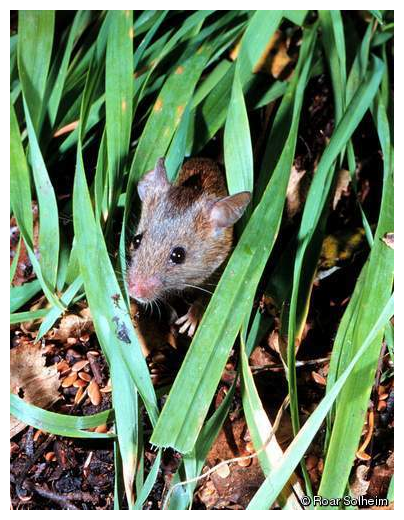
\includegraphics[height=0.2\textheight]{Pics/LC}
                \end{figure}
                VU: vulnerable
                \begin{figure}
                        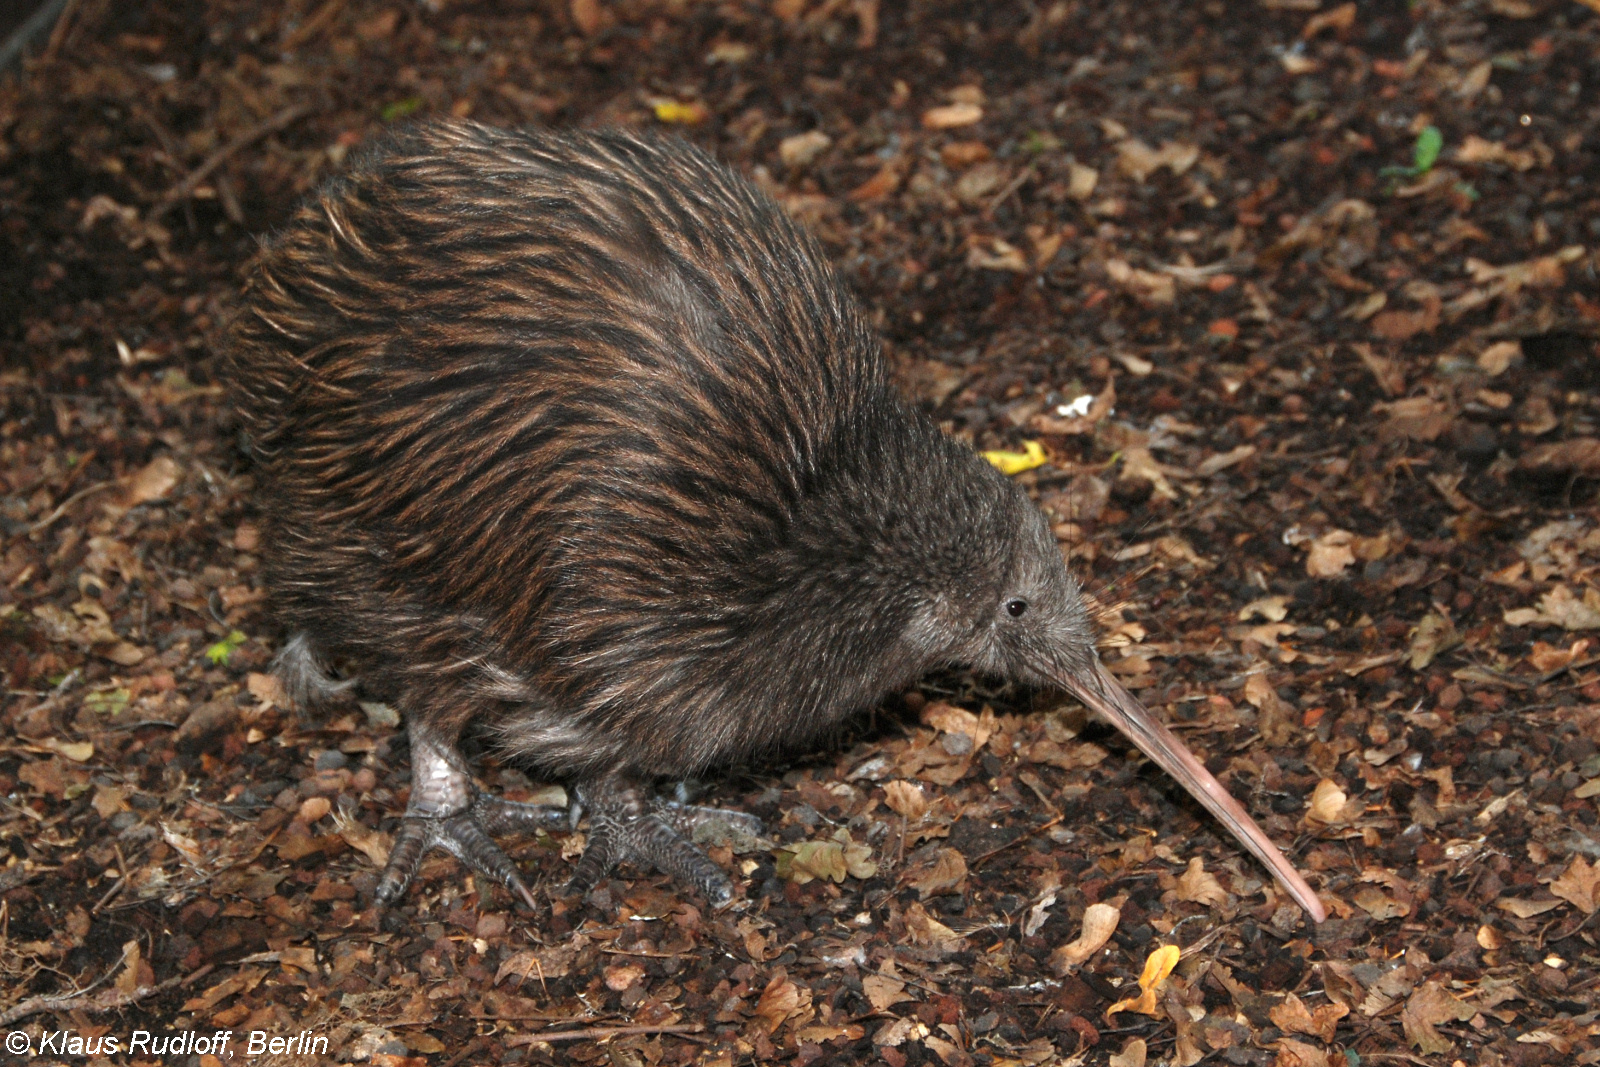
\includegraphics[height=0.2\textheight]{Pics/VU}
                \end{figure}
                \column{0.5\textwidth}
                EN: endangered
                \begin{figure}
                        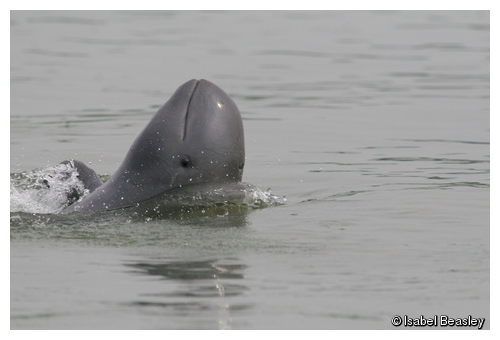
\includegraphics[height=0.2\textheight]{Pics/EN}
                \end{figure}
                CR: critically endangered
                \begin{figure}
                        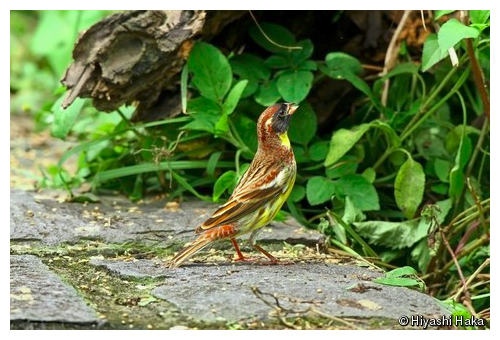
\includegraphics[height=0.2\textheight]{Pics/CR}
                \end{figure}
        \end{columns}

\end{frame}


\begin{frame}
        \frametitle{Population genetics}

        \begin{figure}
        	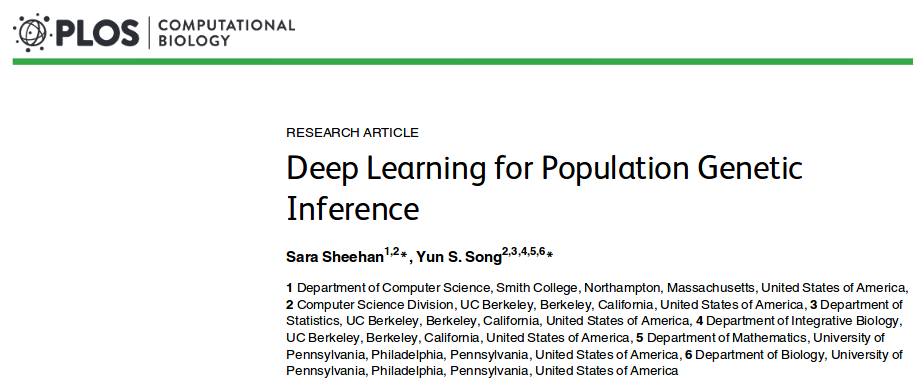
\includegraphics[width=1\textwidth]{Pics/sara.png}
        \end{figure}

\end{frame}

\begin{frame}
	\frametitle{Population genetics}
	
	\begin{figure}
		\centering
		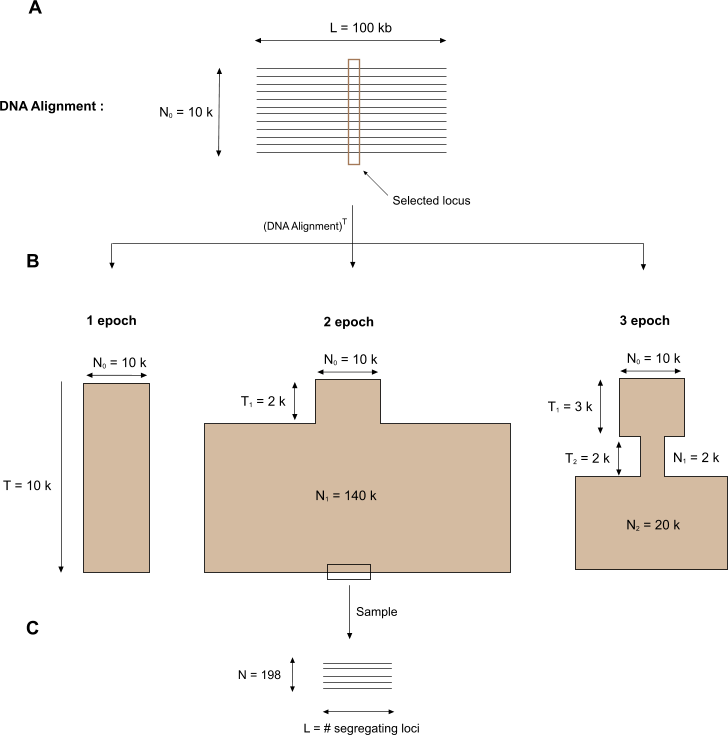
\includegraphics[height=0.8\textheight]{Pics/simulations.png}
	\end{figure}

\end{frame}

\begin{frame}{Genomic data}

	\begin{figure}
    		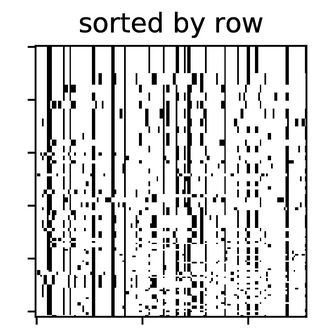
\includegraphics[width=0.4\textwidth]{Pics/example.png}
	\end{figure}

	haplotypes/individuals on rows, genomic positions on columns

\end{frame}

\begin{frame}{CNN applied to population genomic data}

    \begin{figure}
        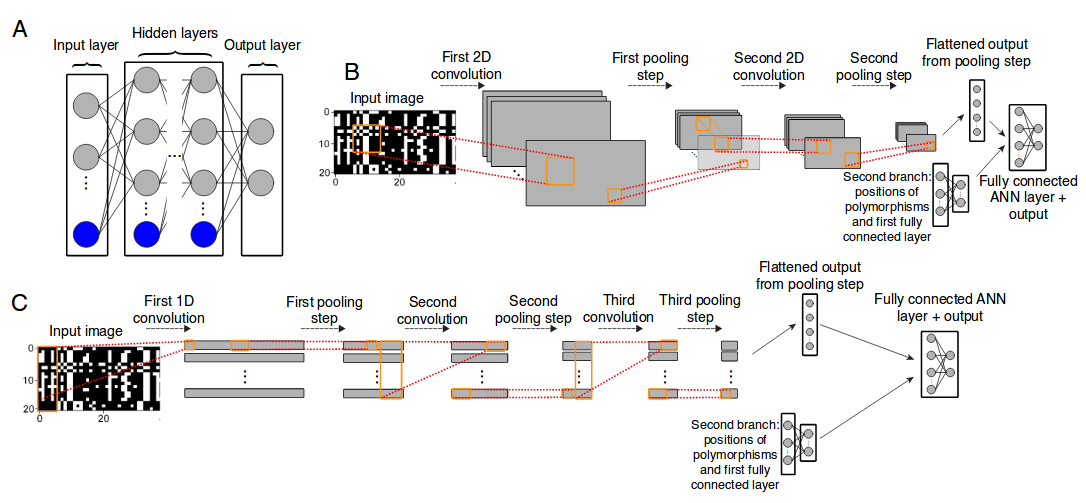
\includegraphics[width=0.9\textwidth]{Pics/flagel.png}
        \end{figure}

\end{frame}

















